This section gives information on pre-fit and post-fit normalizations for 2D analysis at
7 TeV (Table \ref{tab:postnorm_0j_7tev} - \ref{tab:postnorm_1j_7tev}) and 
8 TeV (Table \ref{tab:postnorm_0j_8tev} - \ref{tab:postnorm_1j_8tev}).   
Pull of nuisance paramters are shown in Figure \ref{fig:nuisance_0j_8tev} - \ref{fig:nuisance_1j_7tev}.
Gray region corresponds to input uncertainty($1\sigma$) of each nuiscance.
Solid line indicates the post-fit value(central point) and uncertainty(error bar)
of each nuisance. None of nuisance paramter is shifted more than $1\sigma$ of 
input uncertainty by fit.

%%%%%%%%%%%%%%%%%%%%%%%%%%%%
\begin{table}[ht!]
\begin{center}
\begin{tabular}{c|cc|cc}
\hline \hline
Process     &    N(prefit) &   N(postfit) & Difference(raw) &  Difference(\%)  \\  
\hline \hline
qqH         &        2.9 &        2.1 &       -0.9 &      -29.2        \\
ggH         &      228.1 &      167.5 &      -60.6 &      -26.6        \\
\hline
qqWW        &     3982.2 &     3953.6 &      -28.6 &       -0.7        \\
ggWW        &      211.3 &      285.3 &       74.0 &       35.0        \\
\hline
VV          &      132.6 &      134.6 &        2.0 &        1.5        \\
\hline
Top         &      499.4 &      416.2 &      -83.3 &      -16.7        \\
\hline
Wjets($e$)  &      284.7 &      260.4 &      -24.3 &       -8.6        \\
Wjets($\mu$) &      332.2 &      286.9 &      -45.3 &      -13.6        \\
\hline
W$\gamma$   &      115.6 &      112.5 &       -3.1 &       -2.7        \\
W$\gamma$*  &      130.7 &      132.5 &        1.8 &        1.4        \\
\hline
Ztt         &       44.6 &       45.5 &        0.9 &        2.0        \\
\hline \hline
\end{tabular}
\caption{0-jet bin 8 TeV analysis.}
\label{tab:postnorm_0j_8tev}
\end{center}
\end{table}

\begin{figure}[!hbtp]
\centering 
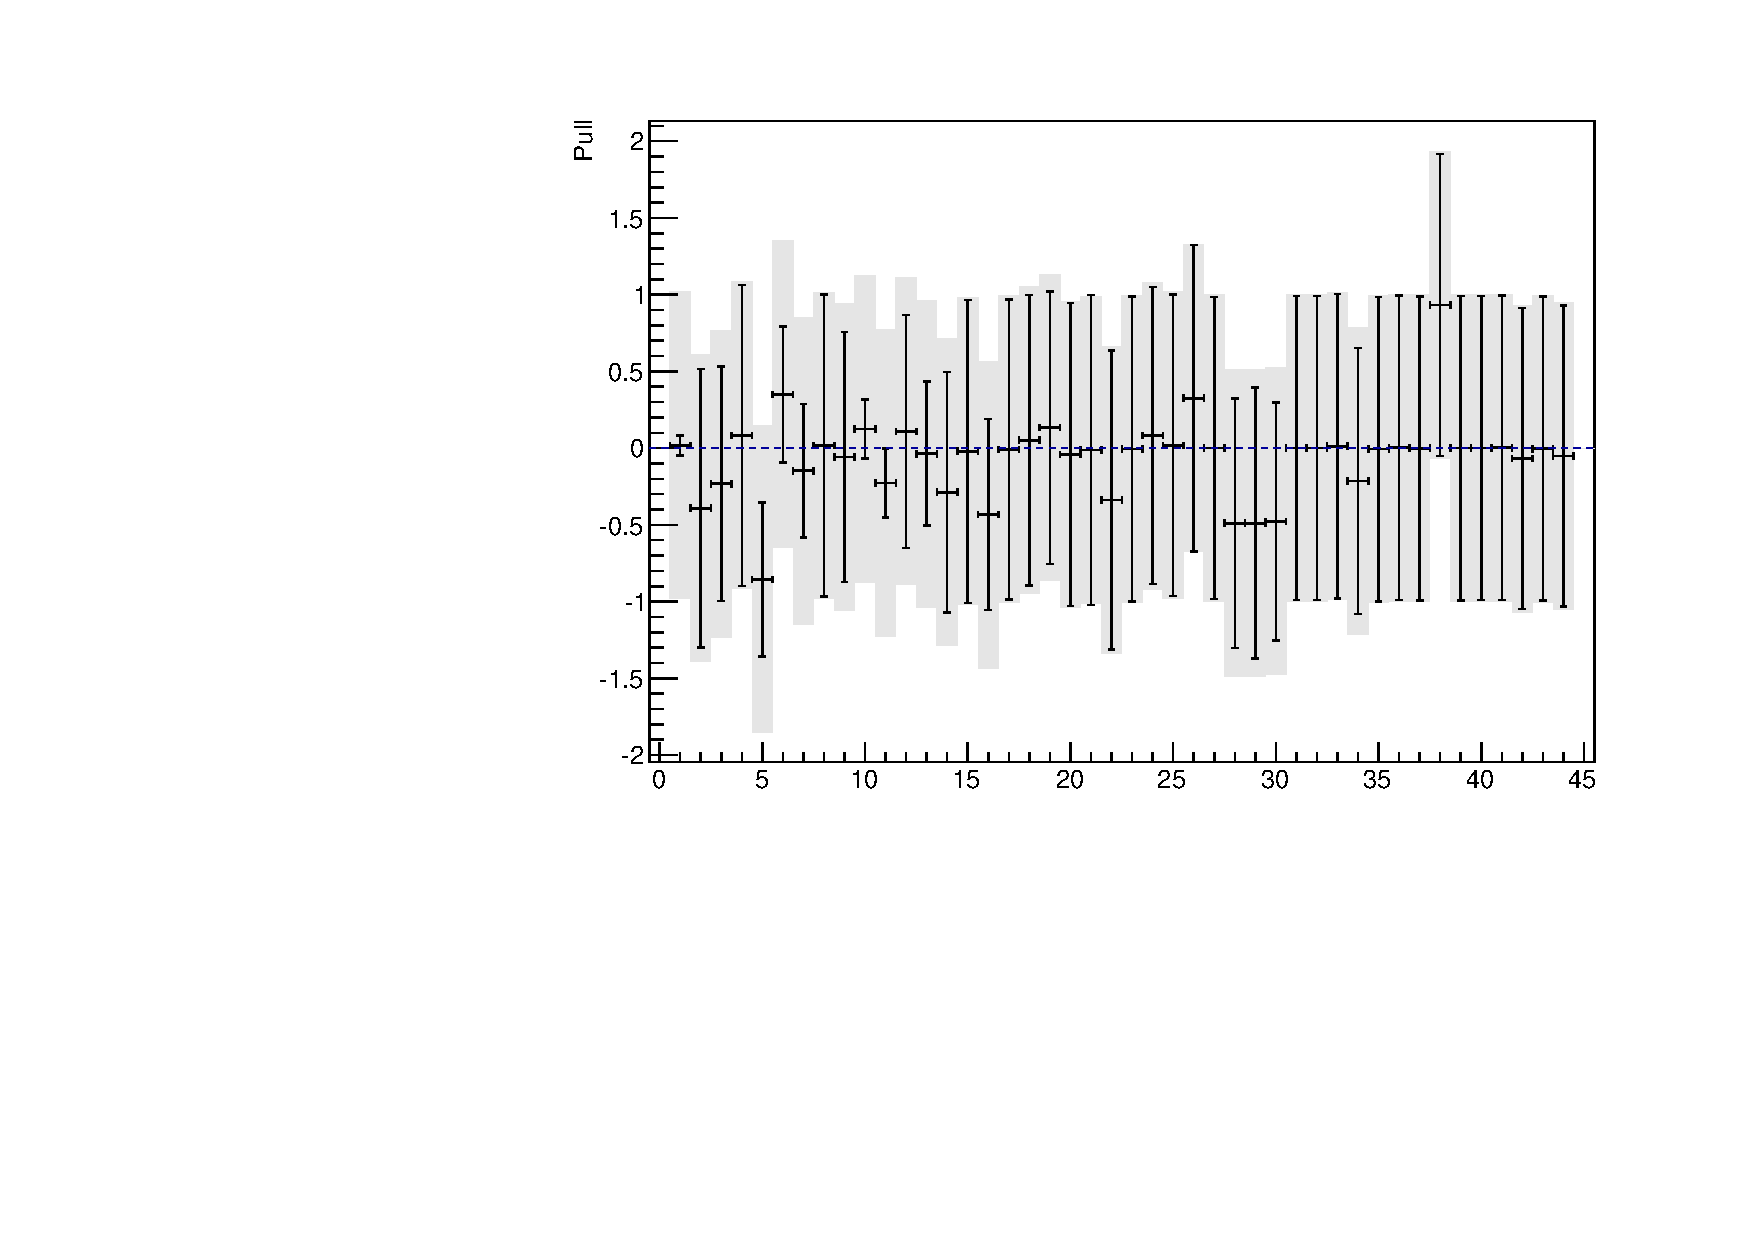
\includegraphics[width=.75\textwidth]{figures/postnuisance_0j_8tev.pdf}
\caption{Pull of nuisance paramters in 0jet bin at 8 TeV.
Gray region corresponds to input uncertainty($1\sigma$) of each nuiscance.
Solid line indicates the post-fit value(central point) and uncertainty(error bar)
of each nuisance.}
\label{fig:nuisance_0j_8tev}
\end{figure} 
\clearpage 

%%%%%%%%%%%%%%%%%%%%%%%%%%%%
\begin{table}[ht!]
\begin{center}
\begin{tabular}{c|cc|cc}
\hline \hline
Process     &    N(prefit) &   N(postfit) & Difference(raw) &  Difference(\%)  \\  
\hline \hline
qqH         &       11.1 &        3.6 &       -7.6 &      -68.0        \\
ggH         &       88.5 &       28.6 &      -59.9 &      -67.7        \\
\hline
qqWW        &     1206.8 &     1354.4 &      147.6 &       12.2        \\
ggWW        &       69.2 &       76.1 &        6.9 &        9.9        \\
\hline
VV          &      116.6 &      115.8 &       -0.8 &       -0.7        \\
\hline
Top         &     1437.1 &     1312.5 &     -124.6 &       -8.7        \\
\hline
Wjets($e$)  &      130.4 &      145.8 &       15.4 &       11.8        \\
Wjets($\mu$) &      153.0 &      154.3 &        1.2 &        0.8        \\
\hline
W$\gamma$   &       29.1 &       30.6 &        1.5 &        5.2        \\
W$\gamma$*  &       20.0 &       12.4 &       -7.5 &      -37.8        \\
\hline
Ztt         &       73.8 &       75.9 &        2.1 &        2.9        \\
\hline \hline
\end{tabular}
\caption{1-jet bin 8 TeV analysis.}
\label{tab:postnorm_1j_8tev}
\end{center}
\end{table}

\begin{figure}[!hbtp]
\centering 
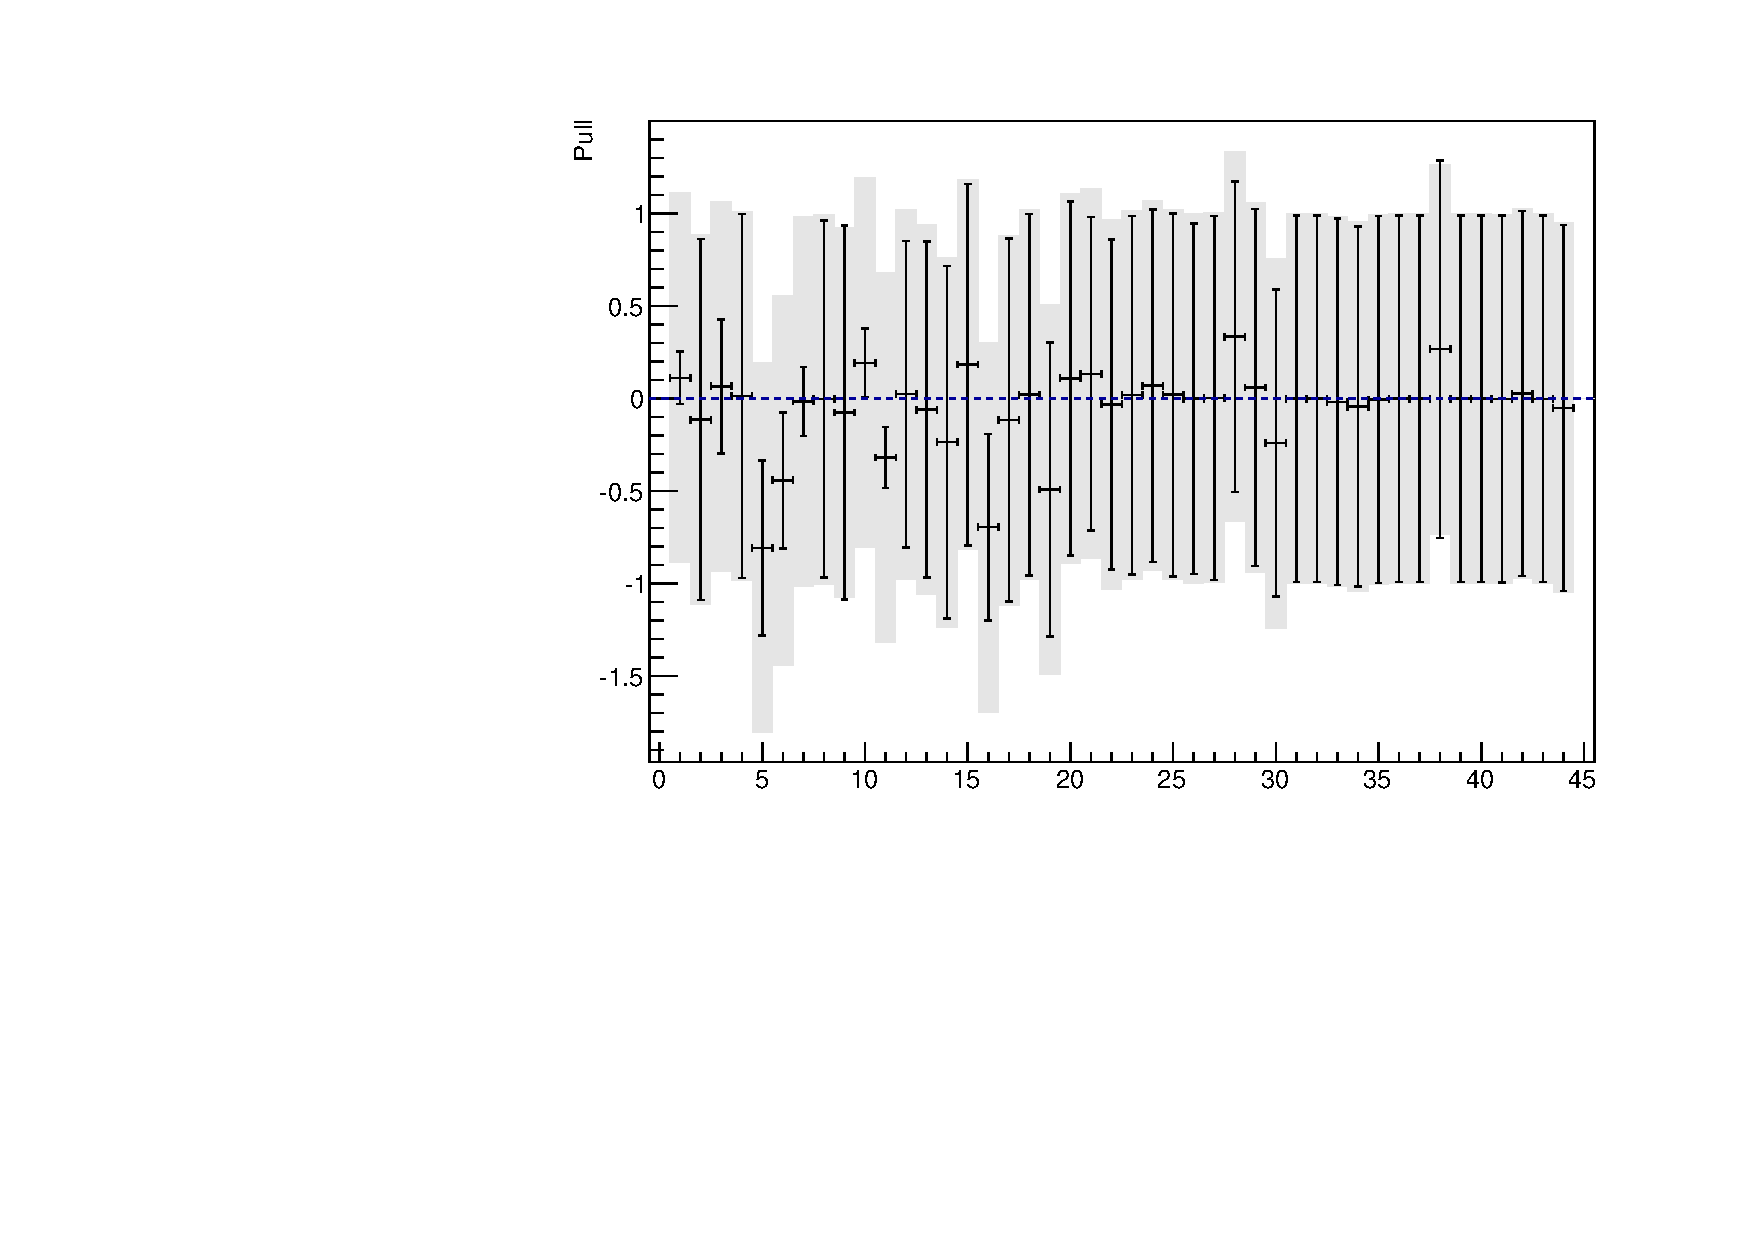
\includegraphics[width=.75\textwidth]{figures/postnuisance_1j_8tev.pdf}
\caption{Pull of nuisance paramters in 1jet bin at 8 TeV.
Gray region corresponds to input uncertainty($1\sigma$) of each nuiscance.
Solid line indicates the post-fit value(central point) and uncertainty(error bar)
of each nuisance.}
\label{fig:nuisance_1j_8tev}
\end{figure} 
\clearpage 

%%%%%%%%%%%%%%%%%%%%%%%%%%%%
\begin{table}[ht!]
\begin{center}
\begin{tabular}{c|cc|cc}
\hline \hline
Process     &    N(prefit) &   N(postfit) & Difference(raw) &  Difference(\%)  \\  
\hline \hline
qqH         &        0.4 &        0.0 &        0.0 &        0.0        \\
ggH         &       50.3 &       32.7 &      -17.6 &      -35.0        \\
\hline
qqWW        &      828.8 &      827.8 &       -1.1 &       -0.1        \\
ggWW        &       40.8 &       38.9 &       -1.9 &       -4.6        \\
\hline
VV          &       17.7 &       17.9 &        0.2 &        1.0        \\
\hline
Top         &       91.2 &       94.1 &        2.8 &        3.1        \\
\hline
Wjets($e$)  &       88.3 &       96.7 &        8.4 &        9.5        \\
Wjets($\mu$) &       62.7 &       60.1 &       -2.6 &       -4.2        \\
\hline
W$\gamma$   &       19.7 &       19.9 &        0.2 &        1.0        \\
W$\gamma$*  &       36.4 &       39.5 &        3.1 &        8.4        \\
\hline
Ztt         &        0.0 &        0.0 &        0.0 &        0.0        \\
\hline \hline
\end{tabular}
\caption{0-jet bin 7 TeV analysis.}
\label{tab:postnorm_0j_7tev}
\end{center}
\end{table} 

\begin{figure}[!hbtp]
\centering 
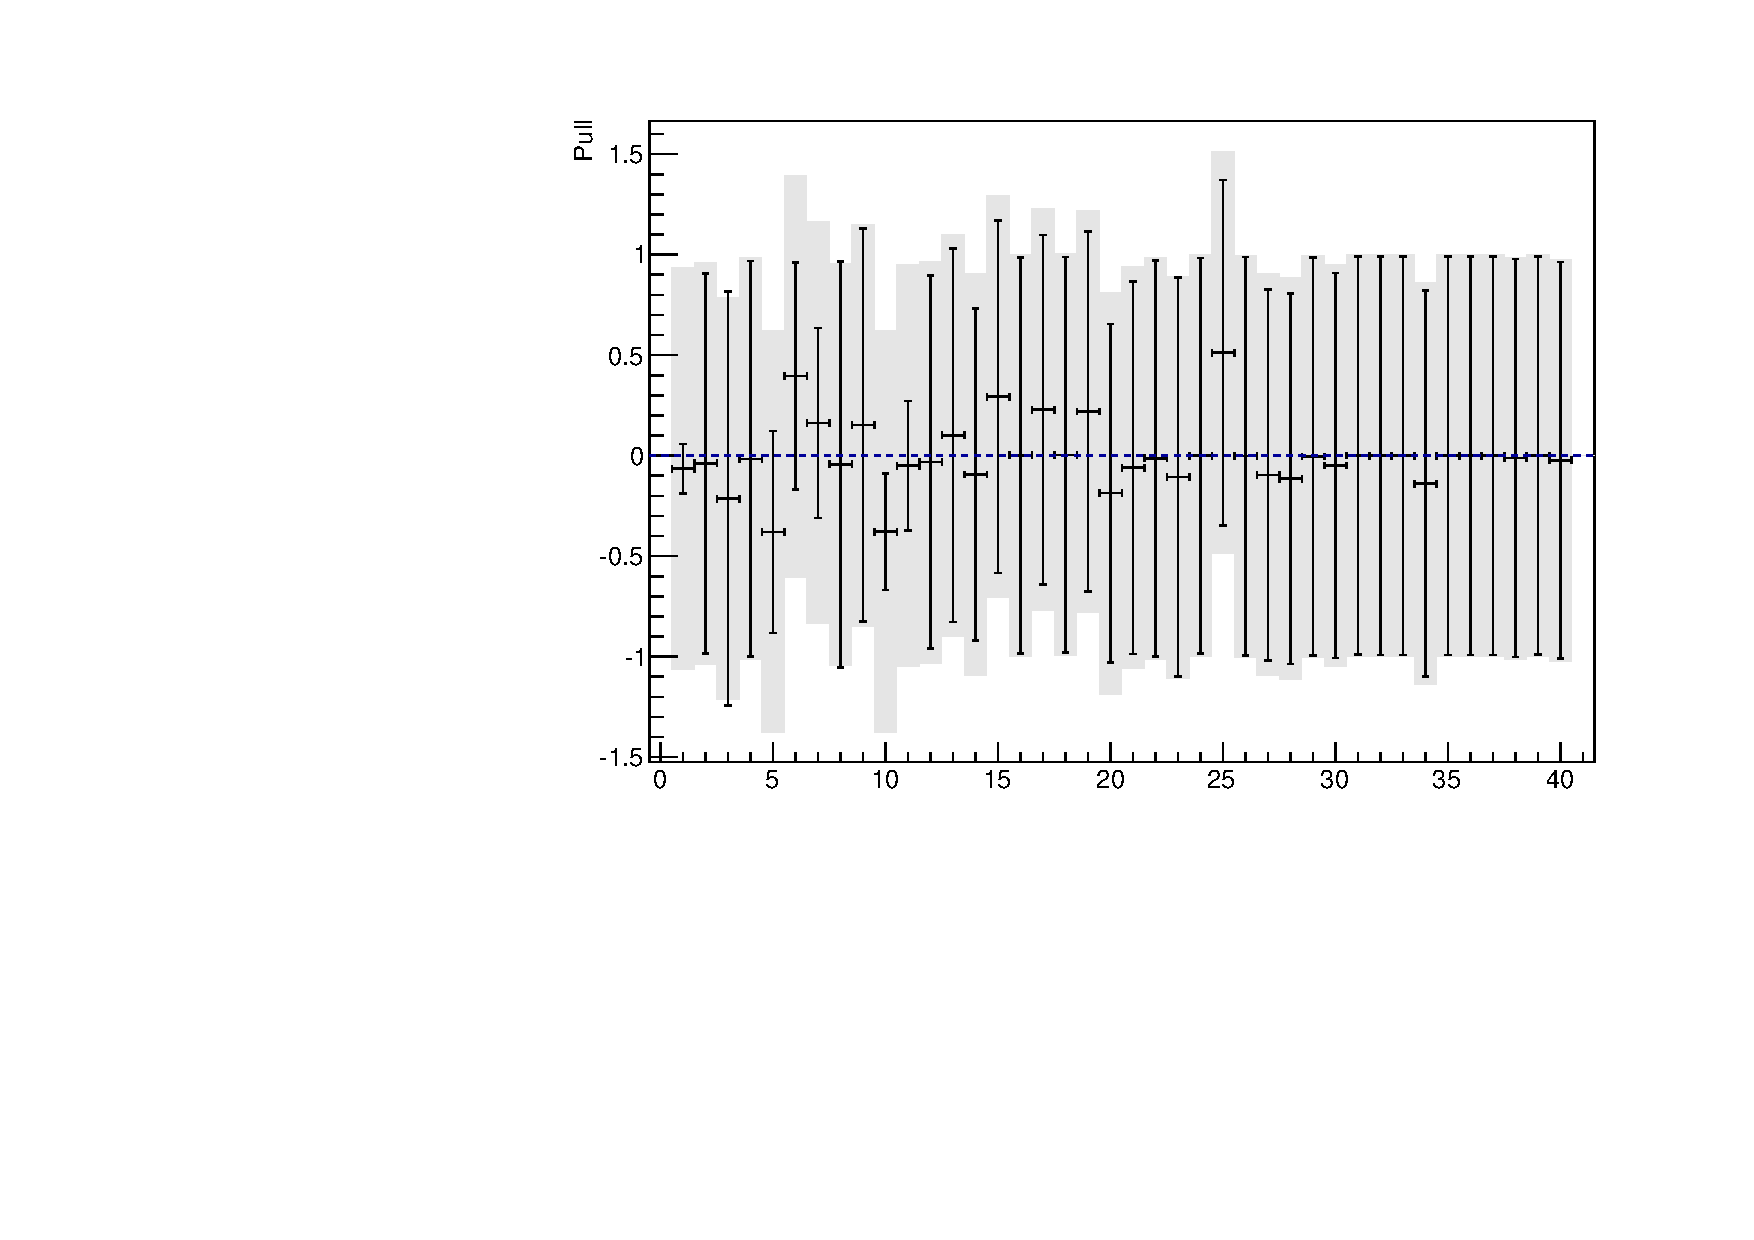
\includegraphics[width=.75\textwidth]{figures/postnuisance_0j_7tev.pdf}
\caption{Pull of nuisance paramters in 0jet bin at 7 TeV.
Gray region corresponds to input uncertainty($1\sigma$) of each nuiscance.
Solid line indicates the post-fit value(central point) and uncertainty(error bar)
of each nuisance.}
\label{fig:nuisance_0j_7tev}
\end{figure} 
\clearpage 

%%%%%%%%%%%%%%%%%%%%%%%%%%%%
\begin{table}[ht!]
\begin{center}
\begin{tabular}{c|cc|cc}
\hline \hline
Process     &    N(prefit) &   N(postfit) & Difference(raw) &  Difference(\%)  \\  
\hline \hline
qqH         &        2.1 &        3.6 &        1.6 &       74.5        \\
ggH         &       17.1 &       32.6 &       15.6 &       91.2        \\
\hline
qqWW        &      246.3 &      277.3 &       31.0 &       12.6        \\
ggWW        &       14.0 &       13.5 &       -0.5 &       -3.6        \\
\hline
VV          &       18.1 &       18.2 &        0.0 &        0.3        \\
\hline
Top         &      226.7 &      200.8 &      -25.8 &      -11.4        \\
\hline
Wjets($e$)  &       34.4 &       29.5 &       -4.8 &      -14.1        \\
Wjets($\mu$) &       26.2 &       19.4 &       -6.8 &      -25.8        \\
\hline
W$\gamma$   &        3.6 &        3.8 &        0.2 &        5.4        \\
W$\gamma$*  &        4.8 &        6.0 &        1.2 &       25.4        \\
\hline
Ztt         &        0.0 &        0.0 &        0.0 &        0.0        \\
\hline \hline
\end{tabular}
\caption{1-jet bin 7 TeV analysis.}
\label{tab:postnorm_1j_7tev}
\end{center}
\end{table}

\begin{figure}[!hbtp]
\centering 
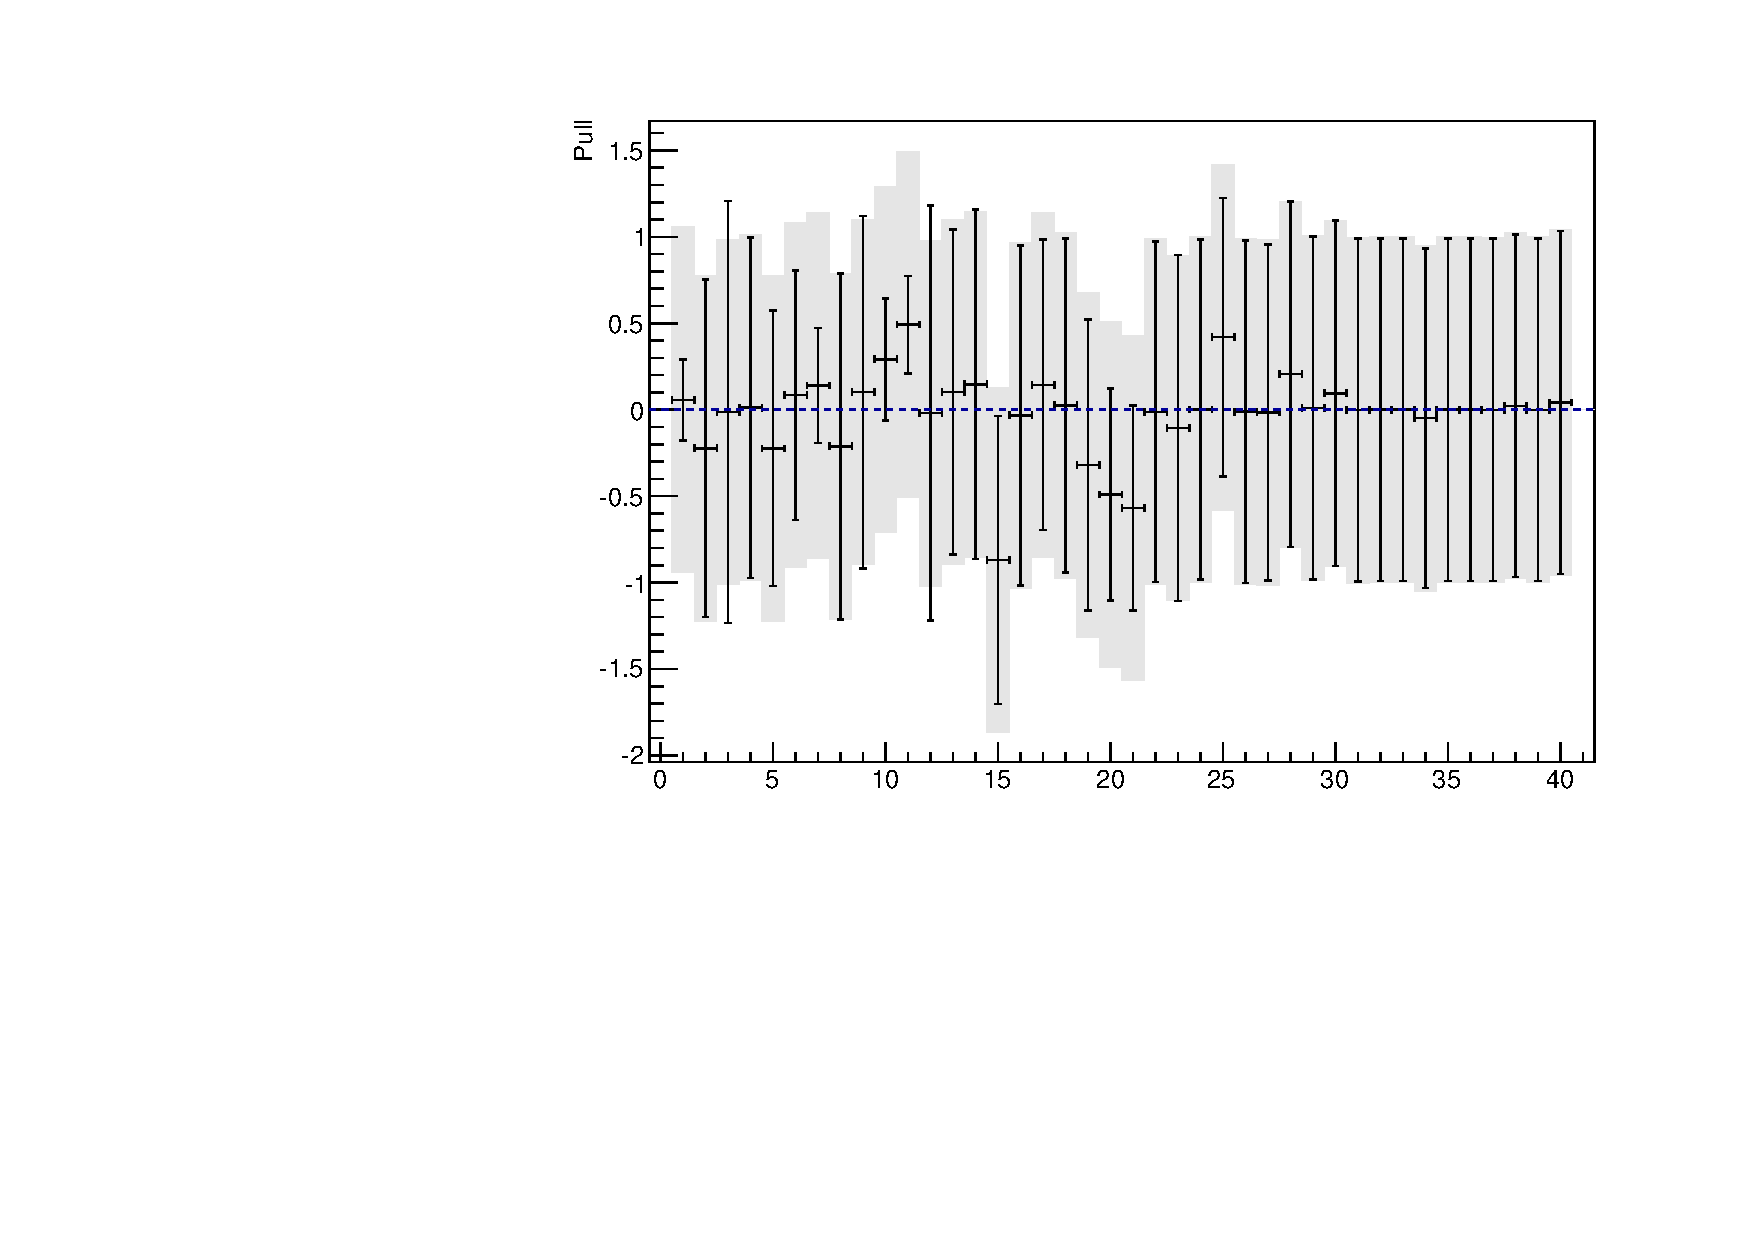
\includegraphics[width=.75\textwidth]{figures/postnuisance_1j_7tev.pdf}
\caption{Pull of nuisance paramters in 1jet bin at 7 TeV.
Gray region corresponds to input uncertainty($1\sigma$) of each nuiscance.
Solid line indicates the post-fit value(central point) and uncertainty(error bar)
of each nuisance.}
\label{fig:nuisance_1j_7tev}
\end{figure} 
